\section{Problem 2 - Quasi-Fermi Levels and Carrier Lifetime}
\textbf{Consider an n-doped Si sample with \( N_{D}=10^{15} \mathrm{~cm}^{-3} \).}

\subsection*{a) Calculate the position of the fermi level $E_F$ relative to the intrinsic position $E_i$}
From
\begin{equation*}
    n_{0}=n_{i} e^{\left(E_{F}-E_{i}\right) / k T}
\end{equation*}

we get

\begin{equation*}
    E_F-E_i=kT \ln \frac{n_0}{n_i}
\end{equation*}

Assuming we are at 300K we get

\begin{align*}
    E_F-E_i=8.62\cdot10^{-5}\cdot 300\cdot \ln \frac{10^{15}}{10^{10}}=0.298eV
\end{align*}

\begin{figure}[H]
    \centering
    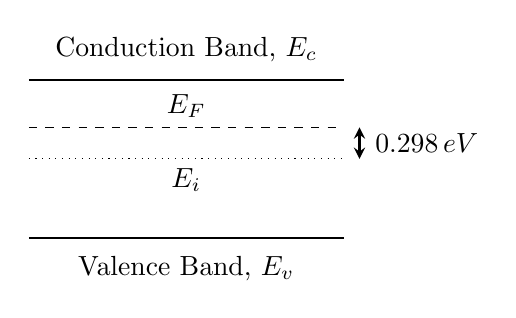
\begin{tikzpicture}[scale=1, transform shape]
    
    % Drawing the energy bands
    \draw[thick] (0,0) -- (4,0) node[midway,above=3pt] {Conduction Band, $E_c$};
    \draw[thick] (0,-2) -- (4,-2) node[midway,below=3pt] {Valence Band, $E_v$};
    
    % Drawing the Fermi and intrinsic levels
    \draw[dashed] (0,-0.6) -- (4,-0.6) node[midway,above] {$E_F$};
    \draw[dotted] (0,-1) -- (4,-1) node[midway,below] {$E_i$};
    
    % Drawing double arrow and label between E_F and E_i
    \draw[<->,>=stealth,thick] (4.2,-0.6) -- (4.2,-1) node[midway,right=2pt] {$0.298 \, \text{eV}$};
    
    \end{tikzpicture}

\end{figure}

\subsection*{b) The sample is steadily illuminated, causing an optical generation rate of \( g_{o p}=10^{19} \mathrm{~cm}^{-3} / \mathrm{s} \). The carrier lifetime is \( \tau_{p}=\tau_{n}=100 \mathrm{~ns} \). Calculate the steady-state carrier concentrations \( n \) and \( p \), as well as the relative positions of the quasi-fermi levels \( F_{n}-E_{i} \) and \( F_{p}-E_{i} \). Compare to the result from a).}

The excess carrier concentration can be written as 

\begin{equation*}
    \delta n=\delta p=g_{op}\tau_n
\end{equation*}

this gives us 

\begin{equation*}
    \delta n=\delta p=10^{19}\cdot10^{-7}=10^{12}cm^{-3}
\end{equation*}

The steady-state carrier concentrations $n$ and $p$ can be written as

\begin{align*}
    n&=n_0+\delta n\\
    p&=p_0+\delta p
\end{align*}

Now that the subscripts are removed, we cant use equilibrium equation $n_0p_0=n_i^2$ as $np \neq n_i^2$

\begin{align*}
    n_0&\approx N_D=10^{15}\\
    p_0&=\frac{n_i^2}{n_0}=\frac{\left(10^{10}\right)^2}{10^{15}}=10^5
\end{align*}

this gives us
\begin{align*}
    n&=10^{15}+10^{12}\approx10^{15}\\
    p&=10^5+10^{12}\approx 10^{12}
\end{align*}

from 

\begin{equation*}
    n=n_ie^{\frac{F_n-E_i}{kT}}
\end{equation*}

we get

\begin{align*}
    F_n-E_i&=kT \ln \frac{n}{n_i}\\
    F_n-E_i&=0.0259 \ln \left(\frac{10^{15}}{10^{10}}\right)\\
    F_n-E_i&=0.298eV
\end{align*}

using 

\begin{equation*}
    p=n_ie^{\frac{E_i-F_p}{kT}}
\end{equation*}

we get
\begin{align*}
    E_i-F_p&=kT \ln \frac{p}{n_i}\\
    E_i-F_p&=0.0259 \ln \left(\frac{10^{12}}{10^{10}}\right)\\
    E_i-F_p&=0.119eV
\end{align*}

\begin{figure}[H]
    \centering
    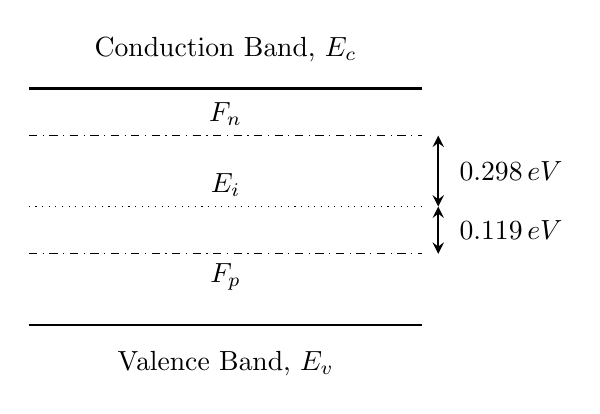
\begin{tikzpicture}[scale=1, transform shape] % Adjusted scale to 1.5 for larger figure

    % Drawing the energy bands
    \draw[thick] (0,0) -- (5,0) node[midway,above=6pt] {Conduction Band, $E_c$};
    \draw[thick] (0,-3) -- (5,-3) node[midway,below=6pt] {Valence Band, $E_v$};

    % Drawing the Fermi and intrinsic levels
    \draw[dotted] (0,-1.5) -- (5,-1.5) node[midway,above] {$E_i$};

    % Drawing the quasi-Fermi levels
    \draw[dashdotted] (0,-0.6) -- (5,-0.6) node[midway,above] {$F_n$};
    \draw[dashdotted] (0,-2.1) -- (5,-2.1) node[midway,below] {$F_p$};

    % Drawing double arrows and labels between levels
    \draw[<->,>=stealth,thick] (5.2,-0.6) -- (5.2,-1.5) node[midway,right=4pt] {$0.298 \, \text{eV}$};
    \draw[<->,>=stealth,thick] (5.2,-1.5) -- (5.2,-2.1) node[midway,right=4pt] {$0.119 \, \text{eV}$};

    \end{tikzpicture}
    \caption{Energy band diagram showing Fermi level ($E_F$), intrinsic level ($E_i$), and quasi-Fermi levels ($F_n$ and $F_p$) with their separations.}
    \label{fig:band_diagram2}
\end{figure}

\subsection*{c) Calculate the time it takes from the light is turned off until the hole concentration is $10\%$ higher than its equilibrium value.}

To calculate when the hole concentration $p=1.1p_0=1.1\cdot 10^{5}$ we must find out $\delta p(t)$ 

\begin{equation*}
    \delta p(t)=\Delta p e^{-\frac{t}{tau_p}}
\end{equation*}

as the carrier lifetime is \( \tau_{p}=\tau_{n}=100 \mathrm{~ns} \), and $\Delta p = 10^{5}$ we get 

\begin{align*}
    \delta p(t)&=10^{5} e^{-\frac{t}{10^{-7}}}=1.1\cdot 10^{5}\\
    -\frac{t}{10^{-7}}&=\ln \left(\frac{1.1\cdot 10^{5}}{10^{5}}\right)\\
    t&=\ln \left(\frac{1.1\cdot 10^{5}}{10^{5}}\right)\cdot\left(-10^{-7}\right)\\
    t&=9.53\cdot10^{-9}s
\end{align*}

